\chapter{Learning Programming}
\label{chap:learning-programming}

% TODO: move the chapter descripton into intro/thesis-structure
This chapter describes the current state of the art of teaching programming, both from the view of successful learning systems and from the view of a research on learning programming.

\section{Existing Systems for Learning Programming}
\label{sec:existing-systems}

There are many systems for learning programming.
These systems can be categorized by several criteria:

\begin{itemize}
\item tangibility: computer systems, or physical toys,
\item platform: web, destkop, or mobile,
\item target audience: e.g. children in a class,
\item prerequisites (assumed prior knowledge),
\item content (covered concepts): loops, conditions, variables, etc.
\item programming language (block-based vs textual),
\item type of tasks (e.g. robot in maze, turtle graphics),
\item (?) playing:learning ratio (term: "game-based learning")
\item (intelligent behavovior -- discussed in next chapter),
\item price: free, or paid.
\end{itemize}

The rest of this section describes the most notable systems.
Section \ref{sec:strategies-for-easier-learning} then attempts to extrapolate useful strategies for teaching programming.


\subsection{LightBot}
\label{sec:lightbot}
LightBot%
\footnote{Available at \url{http://lightbot.com/}.}
is a mobile/web application with a fixed sequence of tasks for learning programming
using block-based programming language.
Students create simple programs to control a robot living in a grid world.
The robot can not only walk and turn left and right, but also jump and turn on lights.
Having 5 different basic commands is useful for diversity of easy tasks.
The system covers sequences of commands, procedures, and simple loops via tail-recursion.

\imgW[0.8]{lightbot}{LightBot.}



\subsection{Robozzle}
\label{sec:robozzle}
With a robot on a grid and block-based programming, Robozzle%
  \footnote{Available at \url{http://www.robozzle.com/}.}
  is similar to LightBot;
however, it adds a new feature: colored fields.
Colors can be used in conditional commands,
  which allows for hundreds of diverse tasks,
  including difficult tasks with sophisticated recursion.
Robozzle also allows users to create their own tasks,
  which can be tried and rated by other learners.

\imgW[0.8]{robozzle}{Robozzle.}


\subsection{BlocklyGames}
\label{sec:blockly-games}
Blockly is a popular block-based programming interface.
In contrast to the blocks in LightBot and Robozzle,
Blockly blocks can be assembled in nested control structures.

The main purpose of BlocklyGames%
\footnote{Available at \url{https://blockly-games.appspot.com/}.}
is to provide a demo of possible Blockly usages.
The webpage consists of several simple games, ordered in increasing difficulty.
For example, in the first level, students learn how to compose blocks together as a puzzle,
and in the second level they learn loops and conditions by solving tasks in a maze.
Final level serves as a transition from block-based programming to textual JavaScript programming.
Each game consists of 5-10 tasks, again with fixed ordered by increasing difficulty, with no personalization.
The fixed order enables to use the program from the previous task,
thus gradually build more and more complex programs,
resulting in, for example, sophisticated images in turtle graphics.
\cite{blockly-10-things}.

\imgW{blockly-instruction}{Blockly Games -- second level. %
The screenshot demonstrates a non-ignorable interactive instruction, %
which require to take a described action before it disappears.}


\subsection{Human Resource Machine}
\label{sec:human-resource-machine}
Human Resource Machine%
\footnote{Available at \url{http://tomorrowcorporation.com/humanresourcemachine}.}
is an example of a paid offline computer game for learning programming using block-based programming interface.
Although it is presented as a game,
the player spends nearly all the time solving tasks similar to those in the previously mentioned learning systems.
The sequence of tasks is non-personalized and nearly linear,
with only a few short side branches.
The main difference from the other systems is a slightly different domain:
it uses more low-level programming commands, such as
input, output, move-from, move-to, add, or jump.
% input, output, move-to, move-from, add, sub, jump, jump-nonzero, jump-negative.
The game comes with a debugger, giving a possibility to step through the program.
All elements are explained when they first appear and programming blocks can be explained again simply by dragging the block onto a field with a question mark.

\imgWithFootnote[0.8]{human-resource-machine}{Human Resource Machine}%
{Source: \url{https://tomorrowcorporation.com/humanresourcemachine} (Tommorow Corporation).}


\subsection{Ozobot}
\label{sec:ozobot}
Ozobot%
\footnote{Information available at \url{http://ozobot.com/}}
is a small physical robot
programmable by either a Blockly-based interface,
  or even without a computer
  by drawing lines on a paper and reading them with a color sensor on the robot.
As it does not require ability to read and write
  Ozobot is suitable for even very young children.


\imgWithFootnote[0.8]{ozobot-robot}{Ozobot}%
{Source: \url{https://www.flickr.com/photos/robpegoraro/19464353039}, Rob Pegoraro.}

% TODO: image of Ozobot!
\imgW{ozobot}{%
  Ozobot simulator (available at \url{http://games.ozoblockly.com}) %
  is a Blockly-like interface for creating programs for Ozobot %
  (but the simulater requires the ability to read). %
  It also includes a few prepared tasks.}


\subsection{Problem Solving Tutor}
\label{sec:problem-solving-tutor}
Problem Solving Tutor%
\footnote{Available at \url{tutor.fi.muni.cz}.}
includes a few problem sets for practicing programming,
such as Interactive Python, Robot Karel, or Robotanist.
After each solved task, Problem Solving Tutor shows a recommendation for two next tasks,
with predicted solving time.
According to the authors, showing predicted time to the user serves as a motivational element
-- it poses a suitable challenge to ``overcome oneself''
\cite{pelanek-student-modeling-times}.

\imgW{robotanist}{Robotanist is a variation on the Robozzle, %
offering both easy introductory tasks requiring no previous exposure to programming, %
as well as extremely difficult tasks on sophisticated use of recursion.}


\subsection{Project Euler}
\label{sec:project-euler}
The core of Project Euler%
\footnote{Available at \url{projecteuler.net}.}
is a list of several hundreds of programming problems with one correct answer.
The problems can be solved in any language
and then checked whether the computed answer is correct.
The project is not meant to teach elementary programming,
but rather to hone one’s programming skills;
more complicated tasks even require some knowledge of algorithms and data structures.

\imgW[0.7]{project-euler-progress}{%
Project Euler provides several means of motivation: %
levels (based purely on number of solved tasks), badges %
(e.g. for solving 10 consecutive problems, 50 prime numbered problems, etc.), %
comparison with user’s friends, %
statistics page with several leaderboard (e.g. by country), %
and a special score based on the performance on the most recently published problems.}


\subsection{HackerRank}
\label{sec:hacker-rank}

Online programming contests,
in which people attempt to solve as many problems as possible
in limited time frame of a few hours,
became popular in the last years.
In addition to organizing such contests regularly,
HackerRank%
\footnote{Available at \url{https://www.hackerrank.com/}.}
also provides many training programming tasks for various topics,
from introductory programming to machine learning.
% Solutions are evaluated on a server against a prepared set of test cases with time limits.
In addition to the classic motivation in the form of points, badges and leaderboards, students are motivated to practice to perform well in the competitions,
where they can win some prizes and sometimes even job offers.
HackerRank also helps student to decide on a problem to solve by showing its difficulty according to the author of the task (on a 3-star scale),
as well as success rate among the past submissions.
Furthermore, after solving a task,
a specific recommendation the next task to solve is shown.


\imgW[0.6]{hackerrank}{HackerRank. %
Each task specifies input and output format, including some examples. %
Solution can be written either locally or in the provided online editor.}


\section{Strategies for Easier Learning}
\label{sec:strategies-for-easier-learning}

Learning programming is difficult,
  because it requires
  to adopt algorithmic thinking,
  understand program execution,
  and remember a formal syntax of a programming language,
  all at the same time.
To make learning easier,
  the systems presented in the previous section use diverse strategies,
  including avoiding syntax errors,
  providing visual output
  and showing helpful hints.
Various other strategies were tried in the past;
article \emph{Lowering barriers for Novice Programmers}
  \cite{lowering-barriers}
  provides a detailed overview.


\subsection{Avoiding Syntax Errors}
\label{sec:avoiding-syntax-errors}

A common strategy in the current systems for learning programming is to avoid syntax errors
  by replacing textual programming with a drag-and-drop block-based programming.
There are two basic types of block-based interfaces:
  either there is a square grid defining the program shape
  (often one row per function),
  or the blocks can be nested and assembled freely with no limitation on maximum program length
  (often one vertical stack per function).
Fixed grid is simpler for understanding and manipulation,
  but it does not allow for direct nesting,
  which is a fundamental feature of computer programs.
This restriction is usually overcome by
  combining condition and a command into a single block,
  using recursion instead of loops,
  and replacing nested sequences of commands by a new function.

TODO: the block-based editors are a special case of "structred editors",
idea: editor only allows edits that transform the code from one syntactically correct
program to another (basically working on AST level, edit = transforms to another AST)
(compared to: classical text editors, where the edit can be arbitraty, making the code
not syntactically correct).

// TBA: comparision figure; e.g. Robotanist - fixed grid, Blockly games - nested blocks


\subsection{Potential Drawback of Block-based Interfaces}
\label{sec:potential-drawback-of-block-based-interfaces}
A drawback of using a block-based programming
  is the students' need to later learn a proper textual language anyhow
  to be able to implement more complex programs.
Several controlled experiments were performed to test the hypothesis
  that it is still beneficial to start an introductory programming course
  with a block-based programming,
  even when the students will be writing code later in the course.
While the results of these experiments suggest that block-based interfaces
  might be the better choice for the start,
  they do not provide strong convincing evidence for that,
  because the programming interfaces used in most of the experiments differ in more aspects
  than in just in using blocks instead of text
  \cite{comparing-blocks-text-price2015}.

TODO: REF 5-week high-school experiment, block-based vs. text-based:
- \cite{comparing-blocks-text-weintrop2017}

\subsection{Transition Strategy}
\label{sec:transition-strategy}
Weintrop and Wilensky suggest that the block representation of the code
  should match the underlying programming language
  to which the student is expected to move in the next phase
  \cite{challenges-of-blocks-based-environments}.
However, the readability of the blocks for learners
  and the resemblance to a programming language
  are sometimes conflicting requirements.
Instead of making compromises,
  BlocklyGames progressively change the available set of blocks in each level,
  making them more similar to JavaScript.
In the last level,
  the text on blocks matches the generated JavaScript completely
  \cite{blockly-10-things}.

TODO:
- note: "blending block-based and text-based programming approaches (e.g., Pencil Code
(Bau 2015), Tiled Grace (Homer and Noble 2014), and Greenfoot’s Frame-based editor (Kölling et al.
2015)"


\subsection{Visual Output}
\label{sec:visual-output}

Good learning systems can help students to track a program execution
  by providing a vivid visual representation of the effects of the program
  together with the current state.
This can be achieved naturally for turtle graphics,
  where the whole state is just a position and orientation of the turtle.
Similarly, in simple games, a grid world with a robot
  contains the full information about the current state.
For the simplicity of their visual output,
  turtle graphics and grid world games have become prevalent task types
  in the current systems for learning programming.

// TBA: figures to illustrate the point; figures to show variants of graphical output


\subsection{Instructions and Hints}
\label{sec:instructions-and-hints}

Most systems for learning elementary programming includes instructions
  to explain new concepts, such as loops and conditions.
However, Neil Fraser explains that students ignore instructions,
  no matter how prominent they are \cite{blockly-10-things}.
His solution in BlocklyGames are non-ignorable, actionable instructions,
  which cannot be closed manually by the student;
  they will only disappear once the student perform the action described in the instruction.

BlocklyGames also include additional hints,
  which only appear after a certain time of unsuccessful solving.
Theoretically, it is possible to generate a hint in any state,
  using data of students which have successfully solved the task before
  \cite{generating-hints},
  but these automatic approaches have not been employed in practice;
  instead, a few manually prepared instructions are usually used.


\imgW{lightbot-instruction}{LightBot provides clear and simple interactive instructions.}

\section{Motivation}
\label{sec:motivation}

In addition to employing the teaching strategies mentioned in section \ref{sec:strategies-for-easier-learning},
  it is equally important to create an engaging environment supporting students’ motivation. Common strategies for increasing motivation are:

\begin{itemize}
\item explaining the usefulness of the programming skill,
\item appealing game world, which is nice to look at and fun play with,
\item gamification elements, such as points and badges,
\item social elements, such as possibility to share programs or achievements,
\item creativity and self-expression (possibility to create own programs),
\item appropriate challenge.
%TODO: consider also: feel of power/control; progress/learning
%TODO: connect those to fulfilling common needs such as being recognized etc.
\end{itemize}


\subsection{Game World}
\label{sec:motivation.game-world}
Ideally, game world should appeal to students --
even without tasks to solve,
  it should be an interesting toy to play with.
In such environments, it is possible to assign open-ended tasks,
  or even let the students create whatever they want,
  which works well especially for creative students seeking for self-expression.

// TBA: figures, providing diverse examples of interesting worlds, including several grid worlds and turtle graphics


\subsection{Tasks}
\label{sec:motivation.tasks}
For many students, giving them specific small problems works better
  than large, loosely defined and open-ended tasks.
By solving small problems quickly,
  they get a feeling of progress and learning.
Another advantage of close tasks
  is a more straightforward implementation of gamification features and adaptive behavior.

Small closed tasks result in short programs,
  but their behavior should be still interesting for the students to be satisfied.
To achieve complex behavior,
  a system can either provide students with macro-commands (e.g. to draw a circle)
  or with a skeleton of complex code, with a few gaps to fill in by students.
However, it is important for the students to feel ownership over the code,
  which is especially a concern with a code skeleton.
Solution suggested by Neil Fraser (and implemented in Blockly Games)
  is to make a series of tasks in which the students
  build on their program from the previous task
  \cite{blockly-10-things}.

// TBA: again some examples in a form of figures + descriptions

%TODO: other important aspects: variability


\subsection{Challenge}
\label{sec:motivation.challenge}
For a great learning experience,
  difficulty of the task must match the skill of the student.
If the task it too easy,
  student is not challenged and gets bored.
If the task is too difficult,
  student gets frustrated and desperate.
On the other hand, if the task has appropriate difficulty,
  student is likely to be challenged and focused.
The complete immersion into the task the student is solving at the moment is called
  a state of flow \cite{flow}.
Achieving the state of flow maximizes the learning outcome \cite{adaptive-practice},
  and even increases the long-term level of happiness. % TODO: find a source of this claim
Next chapter describes techniques for estimating student’s skill
  and show how use that estimate for task recommendation.
% TODO: ref the flow diagram below

\begin{figure}[h]
  \centering
  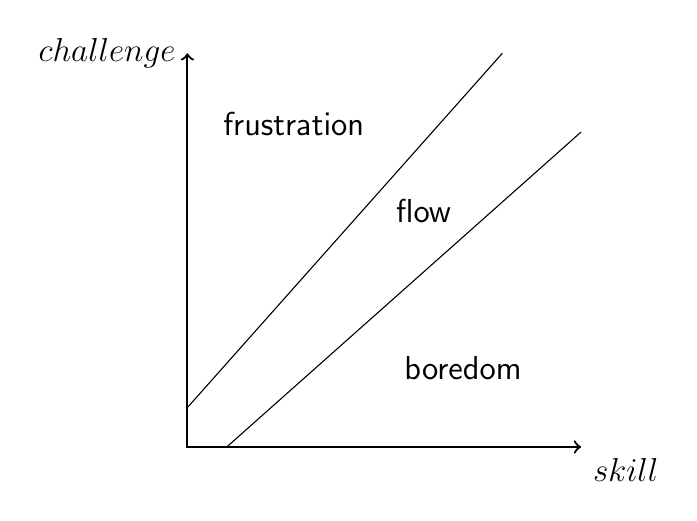
\begin{tikzpicture}[font=\sffamily,xscale=5, yscale=5]
  \large
  %\draw [lightgray, fill=gray] (0,0) -- (0.1,0) -- (1,0.8) -- (0.8,1) -- (0,0.1) -- (0,0);
  \draw (0.1,0) -- (1,0.8);
  \draw (0,0.1) -- (0.8,1);
  \draw [thick, <->] (0,1) node [left] {$challenge$} -- (0,0) -- (1,0) node [below right] {$skill$};
  \node at (0.27,0.82) {frustration};
  \node at (0.6,0.6) {flow};
  \node at (0.7,0.2) {boredom};
  \end{tikzpicture}
  \caption{Relationship between challenge and skill.}
\end{figure}
